\chapter{Introduction} \label{chap1}
\renewcommand{\headrulewidth}{0pt}
\lhead[\thepage]{\leftmark}
\rhead[\leftmark]{\thepage}
\cfoot[]{}

 \section{Context}

 Air pollutants, including nitrogen oxides, carbon monoxide, ozone, and greenhouse gases (GHGs) such as carbon dioxide and methane, are chemical elements present in the atmosphere. These elements have a substantial impact on human health \citep{kampa2008human} and play a role in global warming and climate change \citep{haines2006climate}. Furthermore, these elements are essential components that need to be reduced to foster sustainable development \par

Effectively mitigating the impact of climate change requires a simultaneous reduction in both air pollution and GHGs emissions through the implementation of future policies. The development of impactful strategies to address air pollution is intricately tied to the specific circumstances of each locality, emphasizing the necessity for context-specific approaches. Conversely, the success of GHGs reduction policies relies on a concerted global effort \citep{keohane2011regime}. This is due to the unique characteristics of air pollution and GHGs concerning their residence time in the atmosphere and area of dispersion, as illustrated in Figure \ref{fig:chap1_fig1}.\par

\begin{figure}[tbh!]
    \centering
    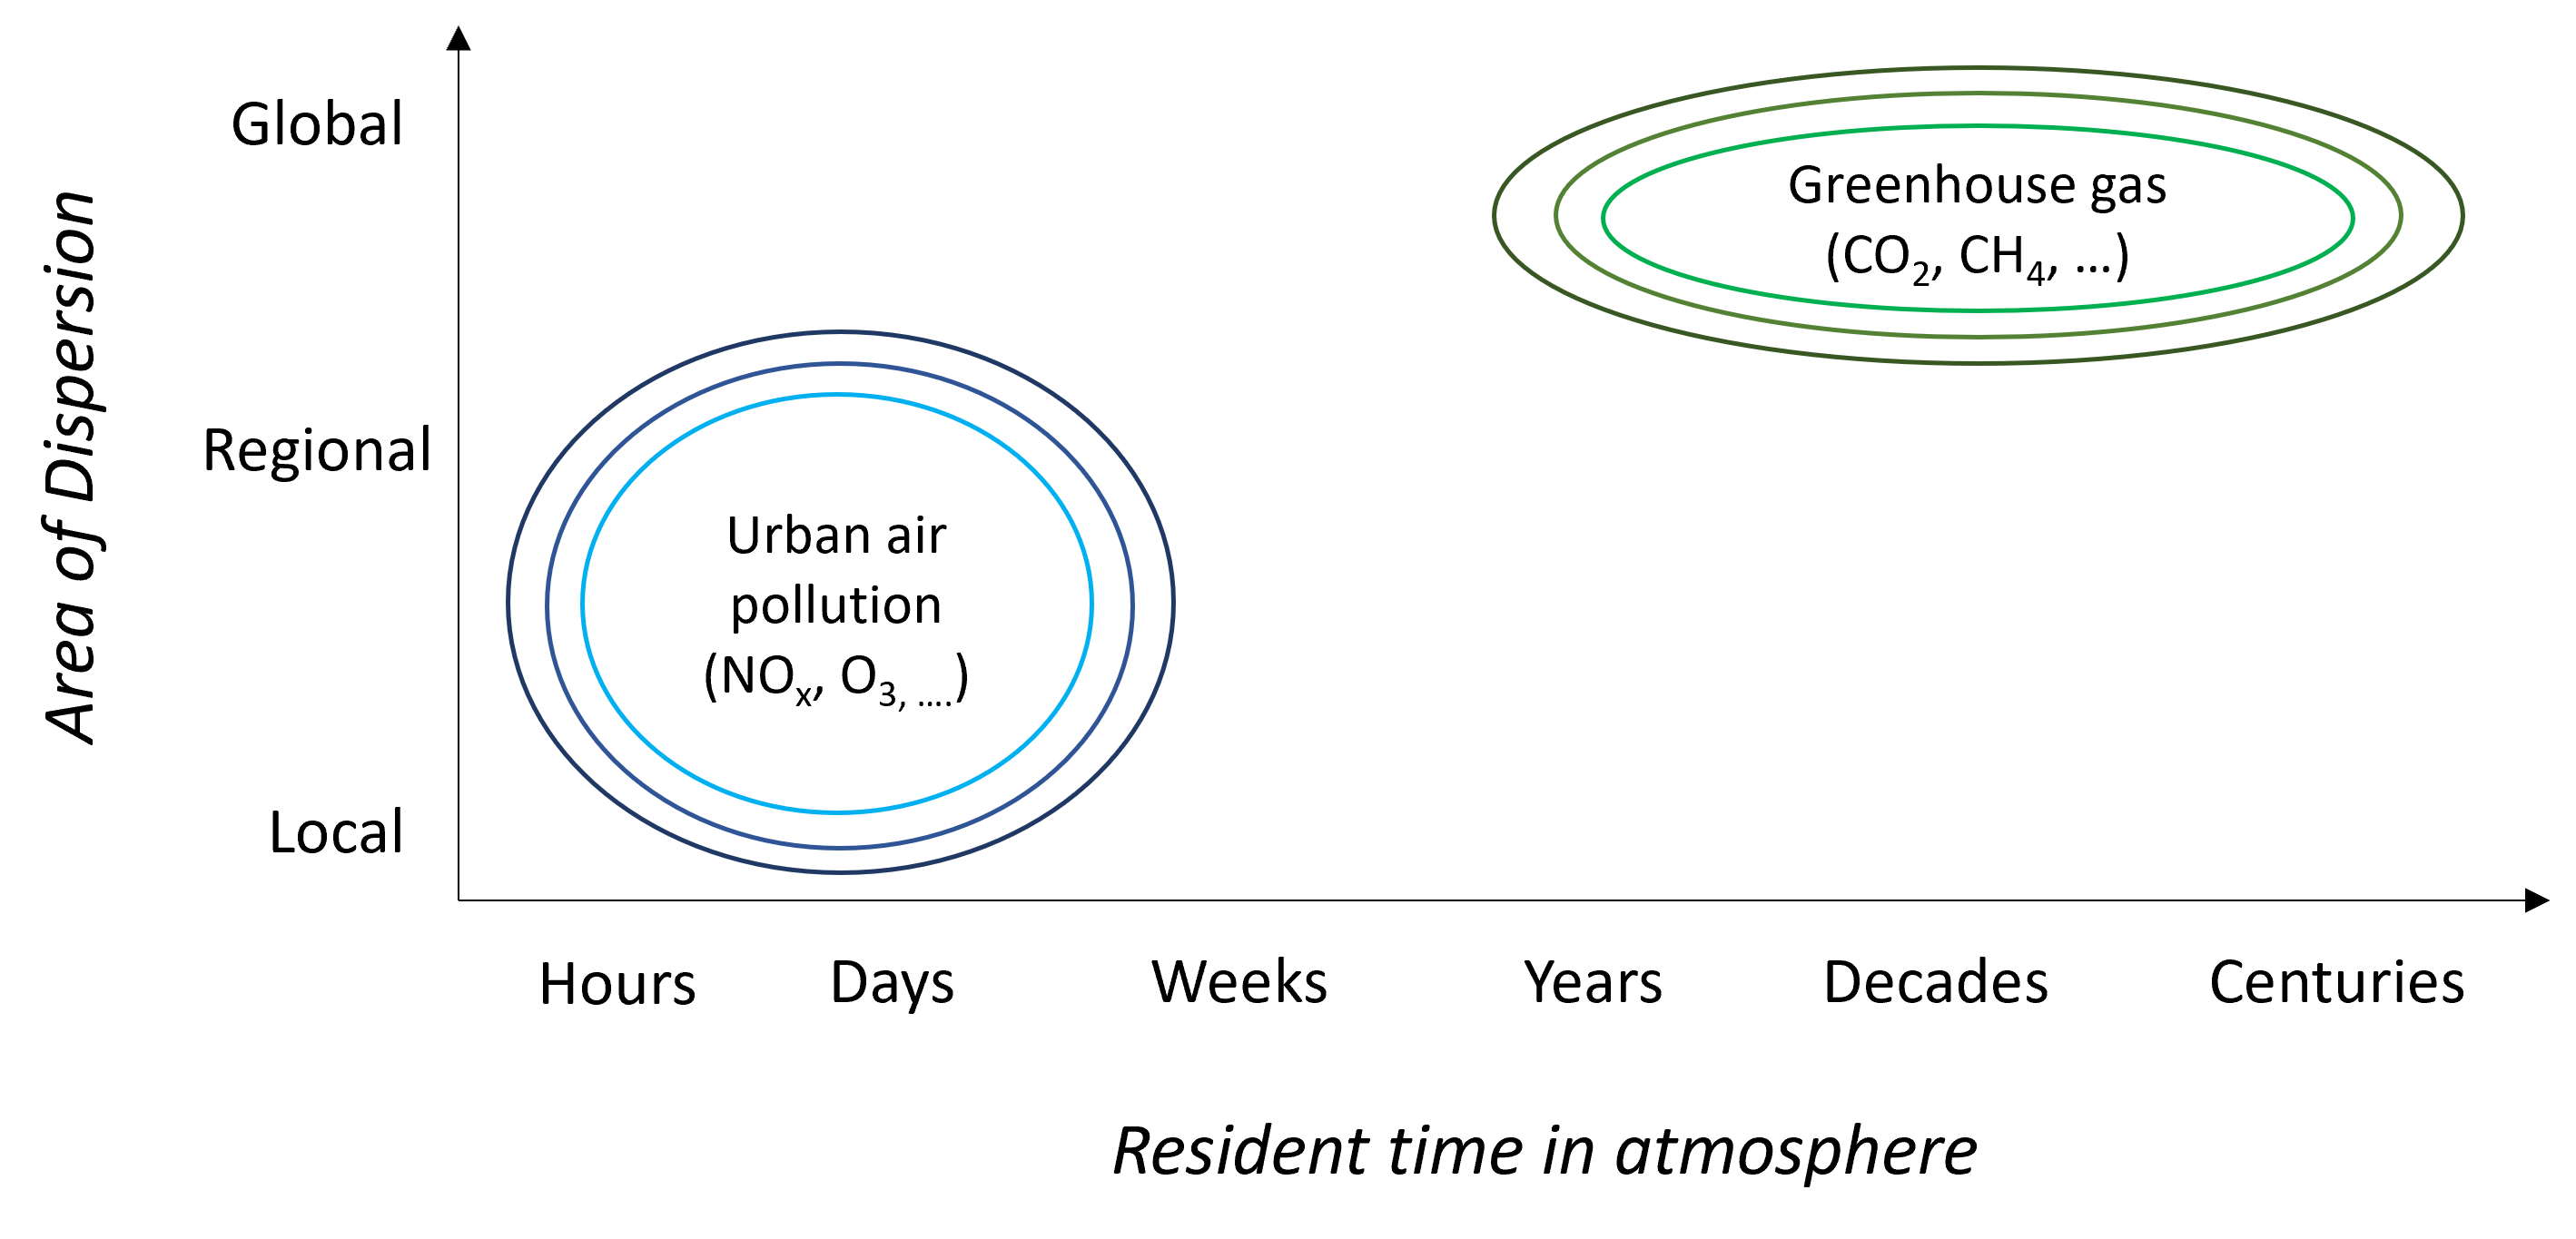
\includegraphics[width=\textwidth]{figs/chap1/residenttime.png}
    \caption[Resident time in atmosphere and the area of dispersion]{Resident time in atmosphere and the area of dispersion of air pollution and GHGs}
    \label{fig:chap1_fig1}
\end{figure}

In the field of air pollution research, the COVID-19 lockdown is viewed as a valuable precedent for shaping future air pollution policies. While the primary objective of the lockdown was not explicitly to address air pollution and GHGs emissions, the adoption of these measures provides valuable insights for atmospheric modeling. This experience imparts practical knowledge and firsthand lessons that can contribute to the development of more efficient strategies for mitigating air pollution and curbing GHGs emissions in the future \citep{grange2021covid}. \par

For zero-carbon emission modeling research, the most critical measure for mitigating the impact of climate change involves a significant reduction in GHGs emissions. One highly effective avenue to achieve this reduction is by enhancing the capacity of terrestrial carbon sequestration, primarily through the preservation and restoration of forests. Notably, between 2010 and 2019, the terrestrial CO\textsubscript{2} sink is estimated to offset fossil CO\textsubscript{2} emissions by 35\%, surpassing the ocean, which is projected to remove 26\% of fossil-fuel-derived CO\textsubscript{2} \citep{friedlingstein2020global, wang2022disentangling}. The substantial global terrestrial carbon flux, known as terrestrial gross primary production (GPP), plays a substantial role in diminishing anthropogenic CO\textsubscript{2} emissions \citep{beer2010terrestrial}. This comprehensive approach not only aids in reducing GHGs levels but also fosters biodiversity and fortifies ecosystem resilience in the face of climate change. \par

While addressing air pollution and GHGs may involve varying levels of collaboration from regional to global scale, the responsibility for monitoring these chemical pollutants is evidently at the local government level. Hence, the necessity of an integrated digital earth platform for air pollution and GHGs monitoring and carbon neutrality roadmaps modelling, as discussed by \citep{fukui2021digital}, is evident for local policymakers to formulate appropriate future policies. \par

\section{Problem statement}
Based on the context of the study described above, this research focuses on three primary themes. The first one directly relates to regional lessons learned from the impact of intervention events, such as the effects of the COVID-19 lockdown on future air pollution policies. The second issue pertains to existing challenges in accurately quantifying the global and local capacity of terrestrial ecosystem carbon flux variables, such as GPP. Lastly, the study concentrates on developing a digital earth platform capable of integrating GHGs emissions monitoring and carbon neutrality roadmaps modelling at the local level, aiming to aid local policymakers in formulating future policies. \par

Concerning the first topic, spanning the period from 2019 to 2022, the world has witnessed two significant intervention events that have profoundly influenced human anthropogenic activities both at local and, to some extent, global levels. The initial event was the COVID-19 lockdown in 2020, followed by the ongoing armed conflict between Russia and Ukraine. These occurrences have led to expected alterations in local and regional air quality, environmental factors, and GHGs emissions. Despite numerous prior studies exploring the impact of the COVID-19 lockdown in many countries, there is considerable variability in results across study areas, as well as in the adopted analytical approaches \citep{shi2021abrupt, grange2021covid}. At the time of our research, to the best of our knowledge, there were limited studies that had thoroughly and comprehensively examined the impact of the COVID-19 lockdown on air pollution in metropolitan areas of Japan. Additionally, there was a scarcity of studies investigating the combined impact of the COVID-19 lockdown and the armed conflict on air pollution in Ukraine, along with the valuable lessons learned for future policy considerations.\par

Regarding the second topic, the estimation of GPP involves a range of methods, including the utilization of dynamic global vegetation models (DGVMs) such as those applied in the TRENDY project \citep{sitch2015recent, le2018global}, as well as upscaling from measurements acquired through eddy covariance (EC) flux towers and satellite observations \citep{jung2019fluxcom, zeng2020global}. However, all these approaches rely on categorizations known as plant functional types (PFTs) to gauge ecosystem productivity \citep{poulter2011plant, poulter2015plant, lin2021improved, guo2023estimating, yan2023integrating}. Discrepancies in PFT maps can introduce significant uncertainties into GPP estimations, as well as other climate-relevant variables, at both regional and global scales \citep{poulter2011plant}. In the tropical region, specifically, challenges arise due to the sparse distribution of EC sites, the high species richness of trees, and the complex vertical structure of tropical rainforests \citep{montgomery2001forest}, making it challenging to accurately quantify the seasonality of carbon fluxes \citep{xu2015satellite}. Recently, there has been a growing adoption of timeseries (TS) foundation models that employ a transformer-inspired architecture for addressing timeseries problems and representation learning. Noteworthy examples include the MVTS Transformer \citep{zerveas2021transformer}, Informer \citep{zhou2021informer}, Autoformer \citep{wu2021autoformer}, and Fedformer \citep{zhou2022fedformer}. The integration of the Transformer architecture is expected to enhance the modeling of seasonality based on the timeseries representation. However, as far as our knowledge extends, its application in the task of upscaling terrestrial global terrestrial carbon fluxes remains limited. \par

The widely recognition of climate change's significance \citep{primack2009impact, watanabe2009general, ogawa2013ecological, shibuya2016effect} is driving an accelerated momentum toward achieving Carbon Neutrality (CN) in local Japanese governments \citep{nakazawa2023net}. Amidst a growing demand for GHGs emissions measurement in corporations \citep{kauffmann2012corporate}, 991 local governments, including Tokyo, Kyoto, and Yokohama, commit to net-zero carbon emissions by 2050 \citep{zerocarboncities}. Achieving this requires comprehensive sector-specific risk analysis and emissions calculation. While local governments integrate map information through Geographic Information Systems (GIS) \citep{nikkei}, separate GIS systems for national energy consumption and power generation as well as forest sinks (local terrestrial carbon fluxes) pose challenges for policymakers \citep{Toshihiko, kitamoto, nlftp}. An integrated WebGIS platform facilitates monitoring and modelling, enabling better understanding and implementation of renewable energy and emission reduction measures. \par
\section{Research questions}
Based the prior problem statements, I am seeking answers to the following questions:

\textbf{Evaluation of intervention events on regional air quality and policy implications}
\begin{itemize}
    \item 1. What was the influence of the COVID-19 lockdown and the armed conflict on air quality in Ukraine, and how can this information offer evidence and recommendations for future policies?
    \item 2. In what ways did the COVID-19 lockdown influence air quality in Japan, and how can this information serve as evidence and provide suggestions for future policies?
\end{itemize}

\textbf{Improved quantification of global terrestrial carbon fluxes}
\begin{itemize}
    \item 3. What methodologies can be employed to improve PFTs mapping performance in data-sparse regions?
    \item 4. Can the utilization of updated PFT maps and Transformer-based models enhance the accuracy of global terrestrial carbon flux estimates?
\end{itemize}
\textbf{Tracking carbon neutrality progress at local level:}
\begin{itemize}
    \item 5. How can we efficiently monitor fossil fuels GHGs emissions as well as the capacity of terrestrial forest carbon fluxes, enabling the development of efficient carbon neutrality roadmaps as well as tracking progress at the local level?
\end{itemize}

\section{Outline of the thesis and scope}

The thesis is structured into six chapters, as depicted in Figure \ref{fig:chap1_fig2}. Chapter \ref{chap2} provides the background on air pollution, GHGs, as well as the interrelationship between these factors themself and with Sustainable Development Goals (SDGs). This chapter also details how this thesis utilizes the digital earth systems approach in each experiment. \par
\begin{figure}[tbh!]
    \centering
    
\includegraphics[width=\textwidth]{figs/chap1/outline.png}
    \caption{Outline of this thesis}
    \label{fig:chap1_fig2}
\end{figure}

In Chapter \ref{chap3}, section \ref{chap3_s1}, I discuss the examination of fluctuations in nitrogen dioxide (NO\textsubscript{2}) levels in Ukraine during two noteworthy periods: the COVID-19 pandemic lockdown in 2020 and the armed conflict with Russia in 2022. In Chapter \ref{chap3}, section \ref{chap3_s2}, I provide an assessment of the impact of alterations in anthropogenic activities during the COVID-19 pandemic (spanning from April 7 to December 31) on NO\textsubscript{2}, O\textsubscript{3}, CO, and CH\textsubscript{4} levels in metropolitan areas of Japan in 2020. \par

In Chapter \ref{chap4}, section \ref{chap4_s1}, I introduced an approach to monitor local forest utilization towards SDGs, focusing on aspects such as PFTs and forest age in data-scarce regions of Japan. In Chapter \ref{chap4}, section \ref{chap4_s2}, I assess the effectiveness of utilizing timeseries representation, particularly leveraging recently updated PFTs and a model based on Transformer architecture, to more accurately quantify seasonal patterns and long-term trends in global terrestrial carbon fluxes. \par

In Chapter \ref{chap5}, I designed a prototype of digital earth platform that facilitates the visualization and support of CO\textsubscript{2} monitoring and the carbon neutrality roadmaps modelling at the municipality level in Japan. \par

Finally, in Chapter \ref{chap6}, I summarize the key findings and contributions of the study and discuss future prospects.\par